\documentclass{beamer}
\usetheme{metropolis}
\usepackage{amsmath}
\usepackage{pifont}
\usepackage[T1]{fontenc}
\usepackage[font=small,labelfont=bf]{caption}
\fontfamily{verdana}\selectfont
\setlength{\unitlength}{\textwidth}  % measure in textwidths
\setbeamercolor{item}{fg=black}
\setbeamertemplate{itemize items}[triangle] % if you want a ball
\setbeamertemplate{itemize subitem}[triangle] % if you want a circle
\setbeamertemplate{itemize subsubitem}[triangle] % if you want a triangle

%************ Title & Author ***********************
\title{Running MSE analysis with the a4a platform}
\subtitle{[subtitle]}
\author{[author] \\ \normalfont {\scriptsize \href{mailto:jdoe@doe.com}{<[email]>}}}
\institute{[affiliation]}
\subject{Fisheries Management}

\begin{document}

%*******************************************
\begin{frame}
\titlepage

\end{frame}

%*******************************************
\begin{frame}
\frametitle{Modular MSE}

\Large \centering What is a modular MSE and how does it help ?

\vspace{1cm}

(hint: think of lego !) 

\end{frame}

%*******************************************
\begin{frame}
\frametitle{The management cycle}

\centering
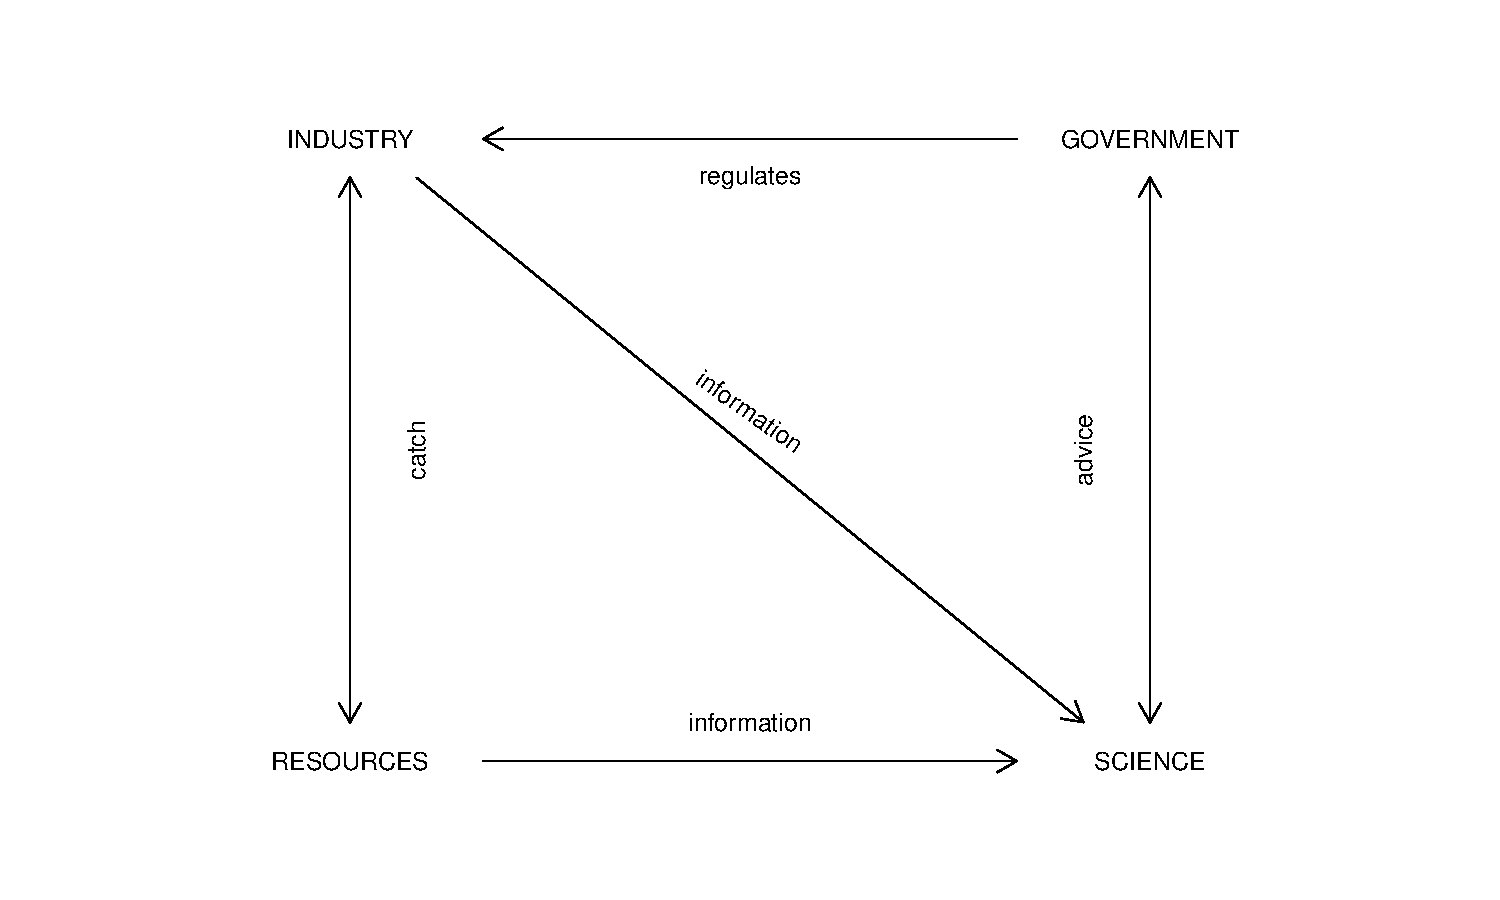
\includegraphics[height=0.8\textheight]{managementCycle2}

\end{frame}

%*******************************************
\begin{frame}
\frametitle{MSE overview}
	
\begin{center}
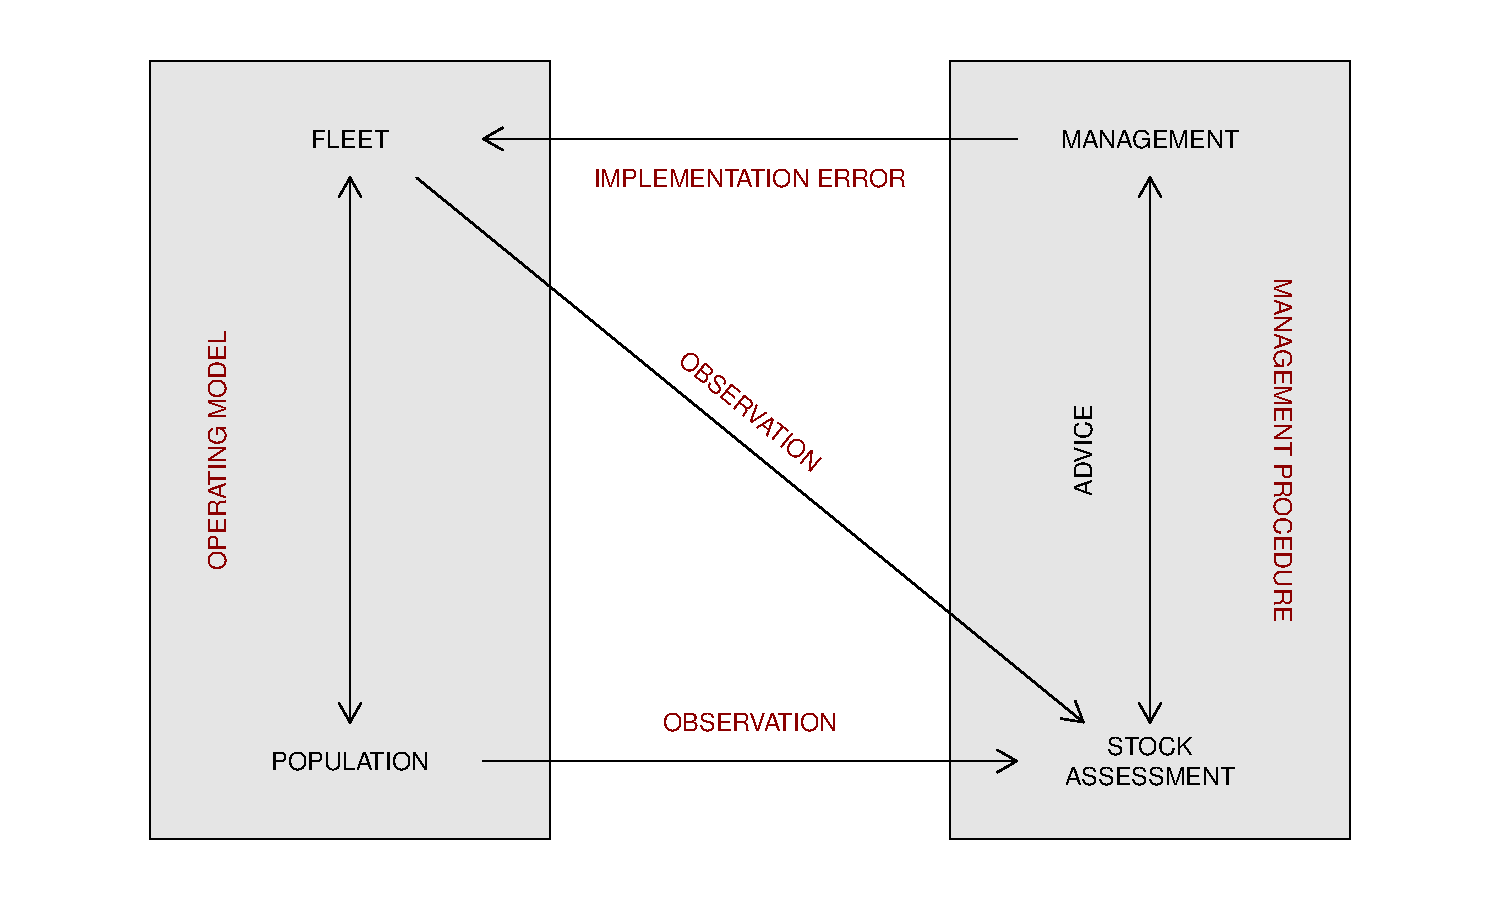
\includegraphics[height=0.8\textheight]{mse}
\end{center}
	
\end{frame}

%*******************************************
\begin{frame}
\frametitle{Generalizing and modularizing the a4a MSE}
	
\begin{center}
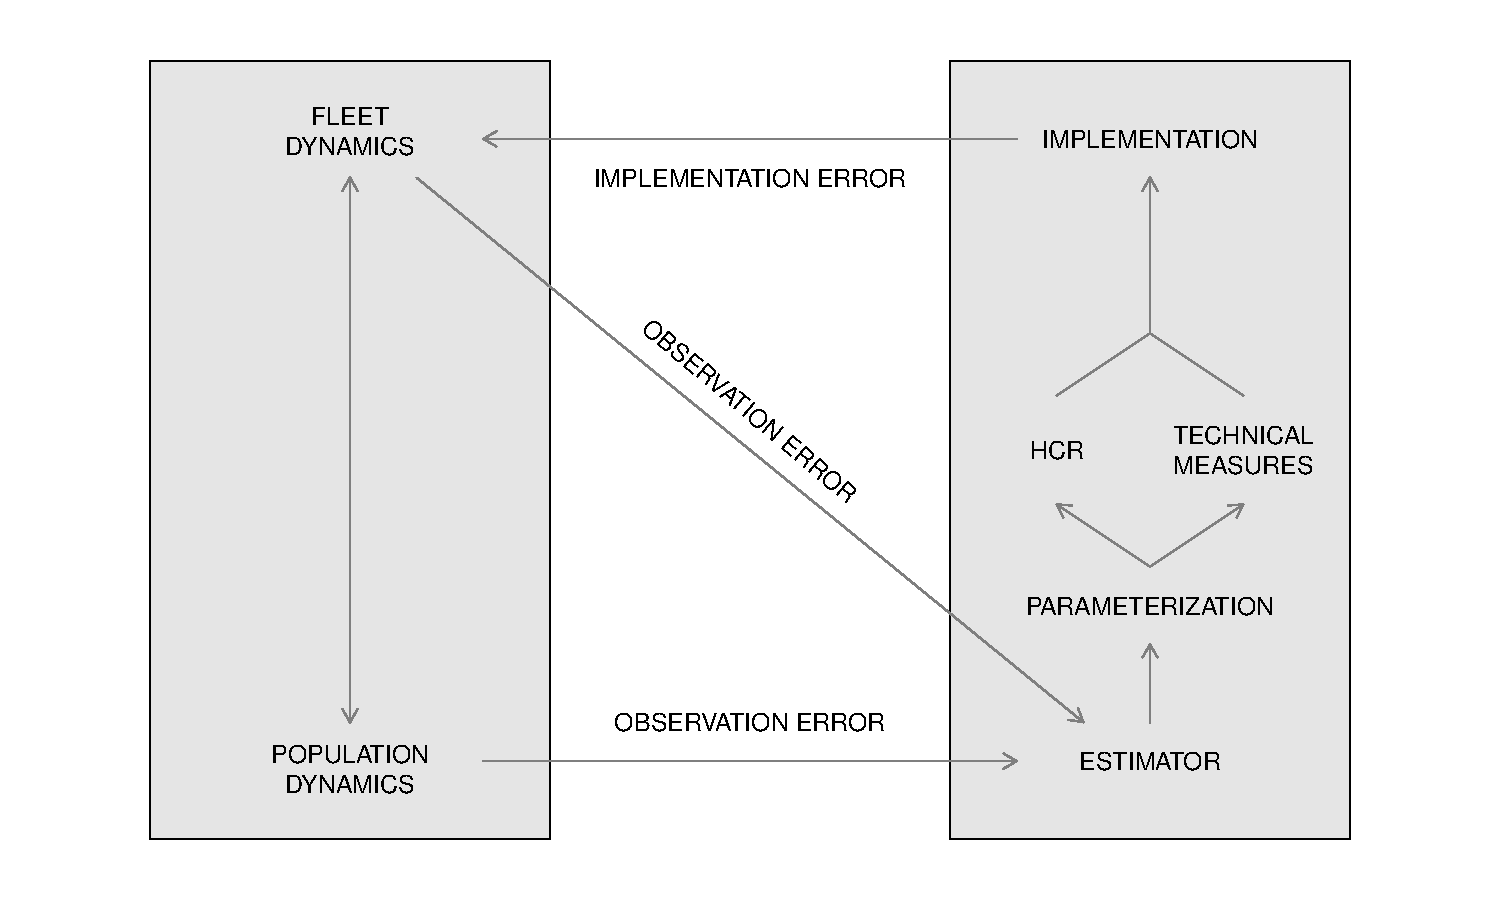
\includegraphics[height=0.8\textheight]{msea4a2}
\end{center}
	
\end{frame}

%*******************************************
\begin{frame}
\frametitle{Timeline}
	
\begin{center}
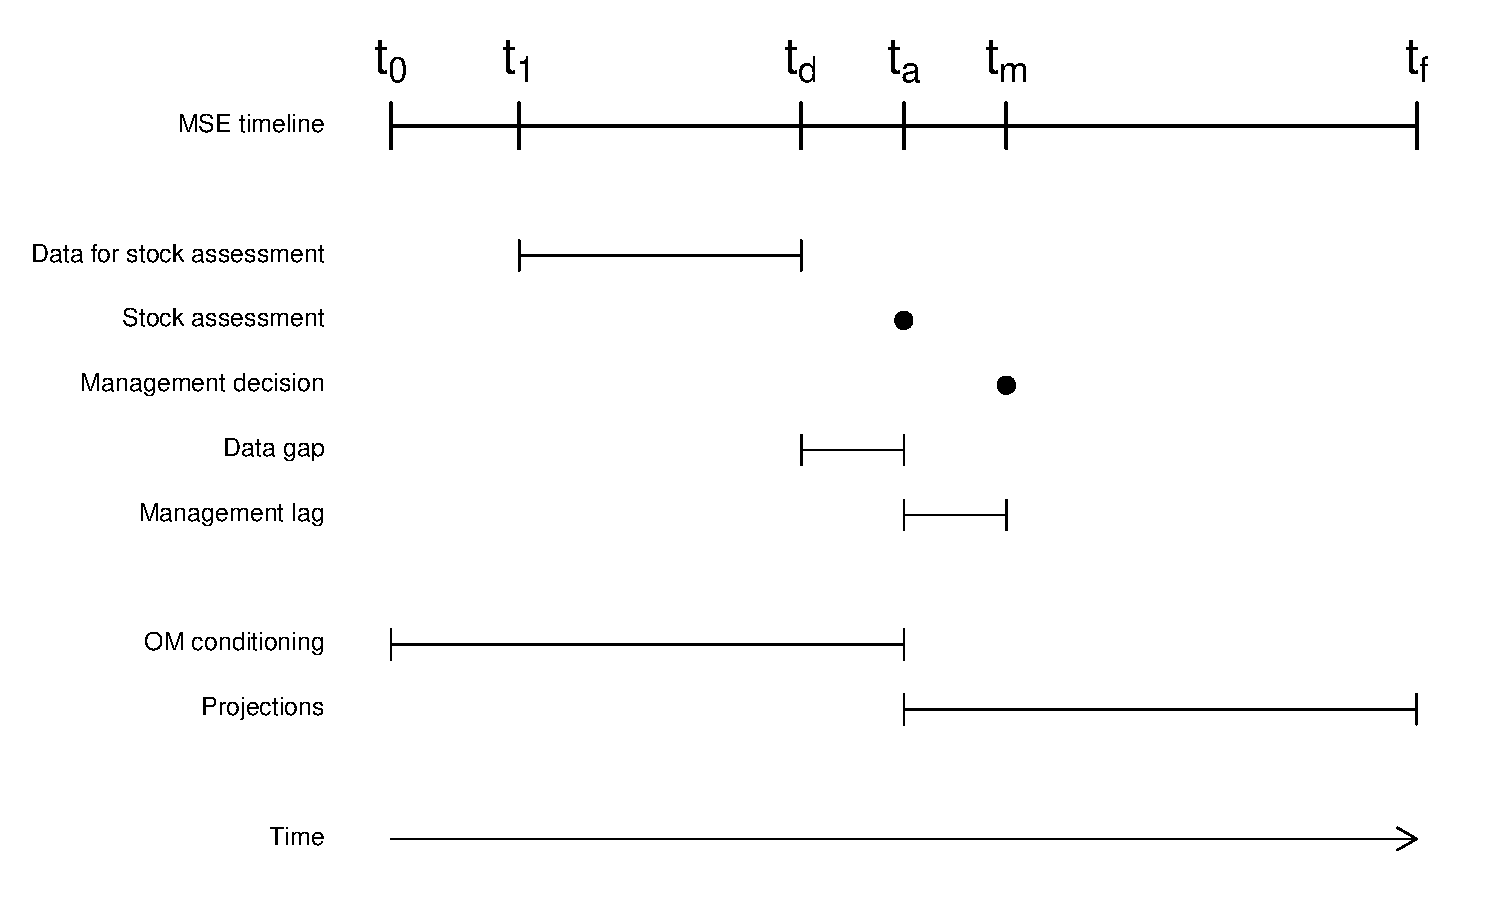
\includegraphics[height=0.8\textheight]{timeline}
\end{center}
	
\end{frame}


%*******************************************
\begin{frame}
\frametitle{Advantages of abstraction}

\footnotesize

\begin{table}
	\begin{tabular}{l|c|c}
		\hline 
		Module	& Data rich & Data limited \\ 
		\hline 
		\hline 
		Observation model	&  catch-at-age, survey & catch length frequencies \\ 
    & & \\
		%\addlinespace[.2cm]
		Estimator	& statistical catch-at-age &  $\bar{L}_{current}$ \\ 
    & & \\
		%\addlinespace[.2cm]
		Parametrization	& $F_{MSY}$ &  $L_{opt}$ \\ 
    & & \\
		%\addlinespace[.2cm]
		HCR	& $F_{future}=F_{MSY}$ & $\delta_{future}=\frac{\bar{L}_{current}}{L_{opt}}$ \\ 
    & & \\
		%\addlinespace[.2cm]
		Technical measures	& [MPA (changes F@age)] & [MPA (changes $\bar{L}_{catch}$)] \\ 
    & & \\
		%\addlinespace[.2cm]
		Implementation	& $TAC=f(C_{past}|HCR)$ & $TAC=f(C_{past} \lor E_{past}|HCR)$ \\ 
    & & \\
		%\addlinespace[.2cm]
		Implementation error	& Uncertainty in catch & Uncertainty in catch \\ 
		\hline 
	\end{tabular} 
	
	\caption{Comparative example of full feedback and data limited MSEs}
\end{table}

\end{frame}

%*******************************************
\begin{frame}
\frametitle{Comments about modular approach}

\Large

\begin{dinglist}{212}
  \item Break large complex system into simpler parts,
	\item Make it simpler to implement and share methods,
	\item Reduces the current workload,
	\item Improves readability, replicability, etc, 
	\item Improves communication !
\end{dinglist}

\end{frame}


%*******************************************
\begin{frame}
	\frametitle{Running MSE analysis with the a4a platform}
	
	\centering Questions?
	
\end{frame}


\end{document}
